\chapter{Evaluation of StencilFlow in Hardware}
We evaluate the performance of StencilFlow on two sets of stencil programs. The first set consists of simple and highly regular kernels, which makes it easy to reason about the measurement and scaling while the second set consists of results from stencil programs of the actual dynamical core.



\section{Experimental Setup}
We performed the evaluation on ault12 consisting of an Intel E5-2630 v4 @ 2.20GHz host CPU with 64GB of RAM and a Nallatech 520N (Intel Stratix 10 GX 2800) FPGA compute card interconnected via PCI-Express. \\
The key specifications of the Nallatech 520N device illustrated in figure \ref{fig:stratix-10} are:
\begin{itemize}
	\item Fast Memory: 25MBytes 
	\begin{itemize}
		\item 11721 M20K (20Kbit) blocks
		\item 23796 MLAB (640bit) blocks 
	\end{itemize}
	\item Host Interface
	\begin{itemize}
			\item 16-lane PCI-Express Gen 3.0 
	\end{itemize}
	\item DDR4 SDRAM Memory
	\begin{itemize}
		\item Four banks of DDR4 SDRAM x 72 bits
		\item 8GB per bank (32GB total)
		\item Transfer Rate: 2400 MT/s 
	\end{itemize}
\end{itemize}
\cite{label60}

\begin{figure}[h]
	\centering
	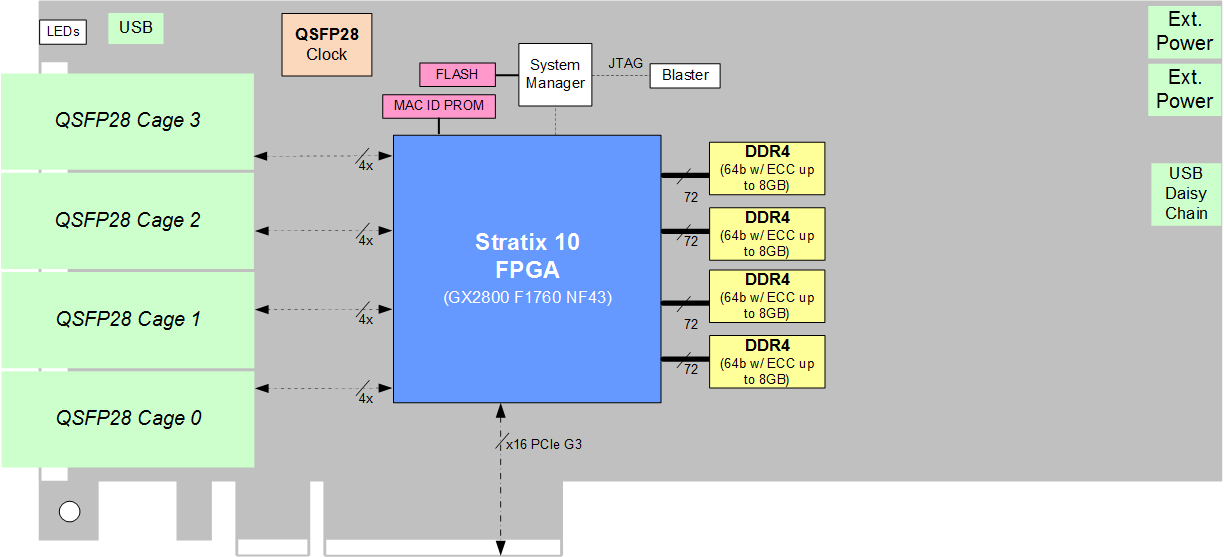
\includegraphics[height=12em]{images/520N.png}
	\caption{Intel Stratix 10 520N Block Diagram, \textit{bittware.com}}
	\label{fig:stratix-10}
\end{figure}
We measured all results 20 times and report the median.


\section{Metrics}
The goal of the evaluation at this point is to find out if our abstracted high-level model of the FPGA corresponds to the actual hardware in different aspects. 

\subsection{Resource Report}
As part of the evaluation, we compare the theoretical usage findings with the values provided in the Intel OpenCL FPGA HLS Report after synthesis of the design. 

\paragraph{Single vs K Iteration}
In order to better understand the the actual scaling of the design, we constructed the Jacobian examples that can easily be scaled in two directions:
\begin{enumerate}
	\item Problem  Size: Scale up the input problem size
\begin{minted}{python}
input: a[1..N]
res = 0.25 * (a[j-1,k] + a[j+1,k] + a[j,k-1] + a[j,k+1])
\end{minted}
	\item Depth: Add many identical stencils after each other. e.g. for K=3:
\begin{minted}{python} 
input: a[1..N]
b[i,j] = 0.25 * (a[j-1,k] + a[j+1,k] + a[j,k-1] + a[j,k+1])
c[i,j] = 0.25 * (b[j-1,k] + b[j+1,k] + b[j,k-1] + b[j,k+1])
res = 0.25 * (c[j-1,k] + c[j+1,k] + c[j,k-1] + c[j,k+1])
\end{minted}
\end{enumerate}



\paragraph{Frequency}
We expect the design frequency to be almost constant throughout the different designs, but since we are not able to directly influence this value, we will add the frequency figures without interpretation if there are no specific outliers. 


\paragraph{LUT}
The number of look-up tables approximately stays constant while scaling up the problem size. We do not model this resource parameter because we assume that LUTs are not the restricting factor.
 
 
\paragraph{FF}
The interpretation of the synthesis report suggests that the number of flip-flops required to build the design is almost constant for a specific design, even when we scale the problem size. We assume that this resource is not the restricting factor.


\paragraph{MLAB}
The number of memory logic array blocks stays constant for a specific design even when we scale the problem size. In addition, it scales linearly with the depth of the problem. We assume that this resource will not limit our design.



\paragraph{RAM}
The random access memory resource is the primary source of fast memory on the device, known as M20K blocks in the Stratix 10 architecture. Since the current implementation of the SDFG generator does not support the actual swap-out of buffers to slow memory, we expect the following relation to hold true: 
\begin{align}
\text{total buffer} = \text{internal buffer + delay buffer} = \text{RAM}
\end{align}
This means that the RAM requirements should scale as follows:
\begin{align}
	\text{buffer requirements in dimensional form} = \text{[a, b, c]}\\
	\text{problem size: [X,Y,Z]}\\
	x + X*b + X*Y*a = c + X*(b  + Y*a)
\end{align}

For the K-Iteration scenario, the buffer requirements are:
\begin{align}
	\text{buffer of K iterations} = K * \text{single iteration}
\end{align}


\paragraph{DSP}
The digital signal processor blocks are processing the actual computation. Since our design is fully pipelined without any parallel execution pipelines, we expect the number of DSP units to stay equal even if we scale the problem dimensions. \\
In the scenario of K-Iterations, we add K such pipelines after each other. Therefore, we expect the number of DSP units to scale linear in K.


\subsection{Execution Time}
In addition to the resource usage, we are interested in how the execution time scales again compared to the problem size and the depth of the problem. 


\paragraph{Single Iteration}
In general, the execution time of a pipeline expressed in cycles is given by
\begin{align}
	\text{execution time} = D + (N-1)*I
\end{align}
where D denotes the depth of the pipeline (latency), I is the number of cycles required to produce an output and N is the actual problem size.


\paragraph{K-Iteration}

The only difference of the K-iteration design is that the depth of the complete pipeline is $K*D$ instead of $D$. Therefore, the formula looks like:
\begin{align}
\text{execution time} = K*D + (N-1)*I
\end{align}



\section{Simple Stencils} 



\subsection{Jacobi2D} 
The first stencil program we analyze consists of a single two-dimensional Jacobian kernel.
\begin{align}    
res = 0.25 * (a[j-1,k] + a[j+1,k] + a[j,k-1] + a[j,k+1])
\end{align}



\paragraph{Frequency}
The design frequency of all problem sizes are between 270Mhz and 325Mhz (figure \ref{fig:jacobi2d_frequency}) as we expected.
\begin{figure}
	\centering
	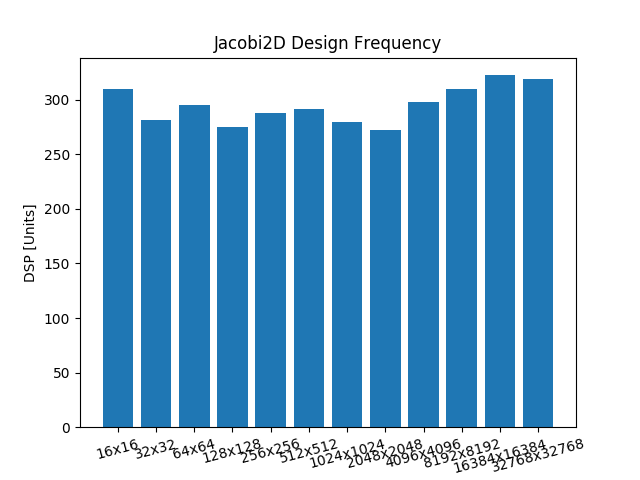
\includegraphics[height=12em]{plots/jacobi2d_frequency.png}
	\caption{Frequency of the high-level synthesized design.}
	\label{fig:jacobi2d_frequency}
\end{figure}



\paragraph{DSP}
The amount of DSP units is constant 3, which  is the number of operations (3 additions and 1 multiplication) of our Jacobian stencil if we assume that one DSP is a fused Add-Multiply unit.
%\begin{figure}[h]
%	\centering
%	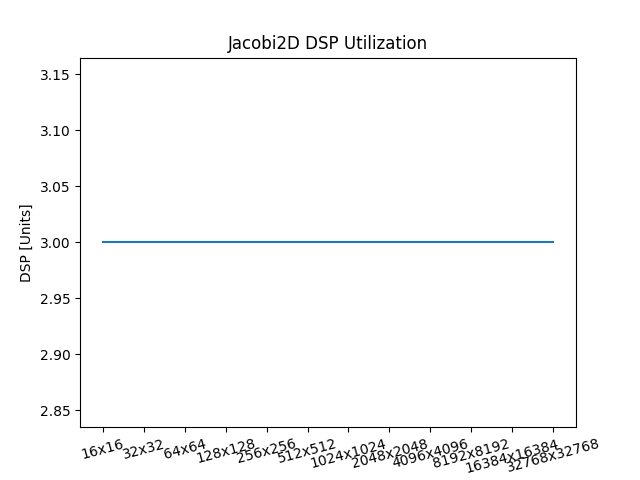
\includegraphics[height=12em]{plots/jacobi2d_dsp.png}
%	\caption{DSP utilization.}
%	\label{fig:jacobi2d_dsp}
%\end{figure}




\paragraph{RAM}
The buffer requirements of Jacobi2D in dimensional form consists of the internal buffer of the kernel only, since a single kernel cannot impose any delay buffers. This is given by $\text{max index} - \text{min index} + 1 = [0, 2, 3]$ which leads to a buffer requirement of
\begin{align}
3 + X*2
\end{align}
This trend of a factor of two by increasing the X dimension by a factor of two too can be seen well for larger  problem sizes in the plot \ref{fig:jacobi2d_ram_comparison}
\begin{figure}[h]
		\centering
		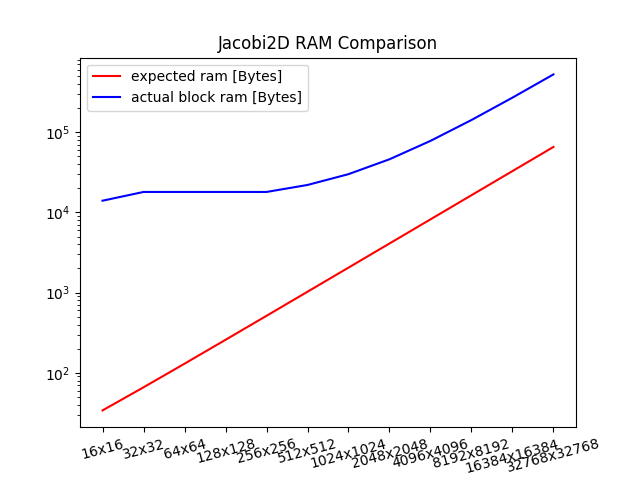
\includegraphics[height=12em]{plots/jacobi2d_ram_comparison.png}
		\caption{Expected buffer size vs block ram usage.}
		\label{fig:jacobi2d_ram_comparison}
\end{figure}


\paragraph{Execution Time}

In general, the execution time of a pipeline expressed in cycles is given by
\begin{align}
\text{execution time} = D + (N-1)*I
\end{align}
By assuming $I=1$  (producing a result every cycle) and using D as the latency computed by StencilFlow which, our estimate is almost perfectly equal to the measurements, especially for larger problem sizes where we can measure more exact.
\begin{figure}[h]
	\begin{minipage}{.5\columnwidth}
		\centering
		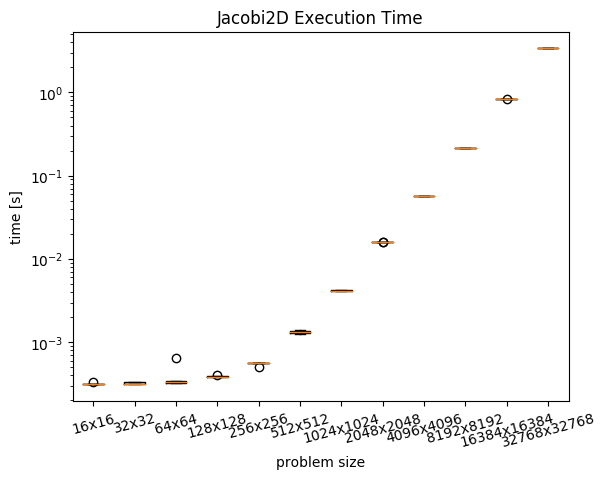
\includegraphics[height=12em]{plots/jacobi2d_execution_time.png}
		\caption{Execution time of Jacobi2D.}
		\label{fig:jacobi2d_execution_time}
	\end{minipage}
	\begin{minipage}{.5\columnwidth}
		\centering
		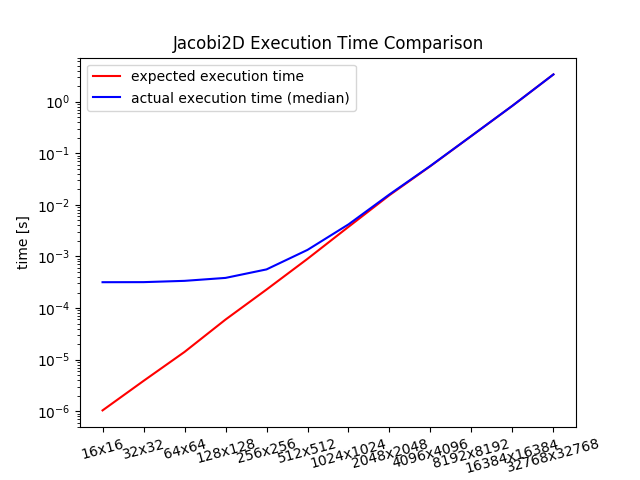
\includegraphics[height=12em]{plots/jacobi2d_execution_time_comparison.png}
		\caption{Expected vs actual execution time.}
		\label{fig:jacobi2d_execution_time}
	\end{minipage}
\end{figure}


\subsection{Jacobi3D} 
The second stencil program we analyze consists of a single three-dimensional Jacobian kernel.
\begin{align}     
res = \frac{1}{6} * (a[i-1,j,k] + a[i+1,j,k] + a[i,j-1,k] + a[i,j+1,k] \notag \\
+ a[i,j,k-1] + a[i,j,k+1])
\end{align}


\paragraph{Frequency}
The design frequency of all problem sizes and iteration depths are between 260Mhz and 330Mhz as we expected.

\begin{figure}[h]
	\begin{minipage}{.5\columnwidth}
		\centering
		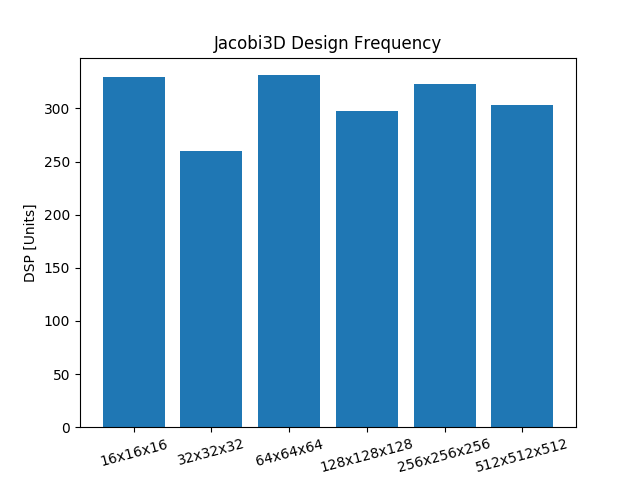
\includegraphics[height=12em]{plots/jacobi3d_frequency.png}
		\caption{Frequency of the high-level synthesized design.}
		\label{fig:jacobi3d_frequency}
	\end{minipage}
	\begin{minipage}{.5\columnwidth}
		\centering
		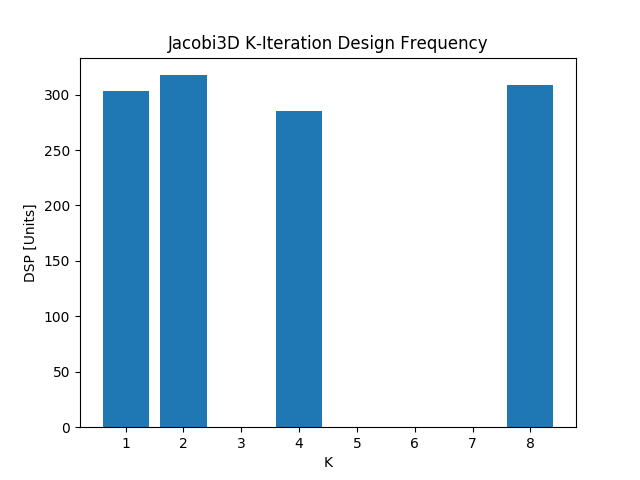
\includegraphics[height=12em]{plots/jacobi3d_k_itr_frequency.png}
		\caption{Frequency of the high-level synthesized design.}
		\label{fig:jacobi3d_k_itr_frequency}
	\end{minipage}
\end{figure}



\paragraph{DSP}

The amount of DSP units is constant six, which  is exactly the number of operations (5 additions and 1 multiplication) of our Jacobian stencil. Furthermore, the value is problem size independent as expected.
%\begin{figure}[h]
%	\centering
%	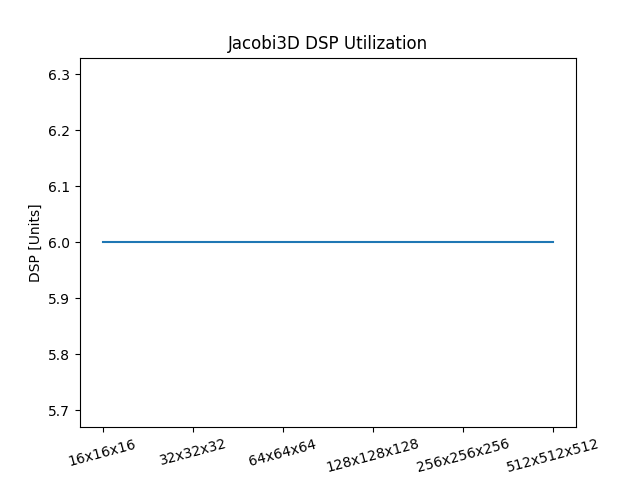
\includegraphics[height=12em]{plots/jacobi3d_dsp.png}
%	\caption{DSP utilization.}
%	\label{fig:jacobi3d_dsp}
%\end{figure}

On the other hand, for the K-Iteration case, the number of DSP units increases perfectly linear with K i.e. 
$K*6$ as shown in figure XY.
\begin{figure}[h]
	\centering
	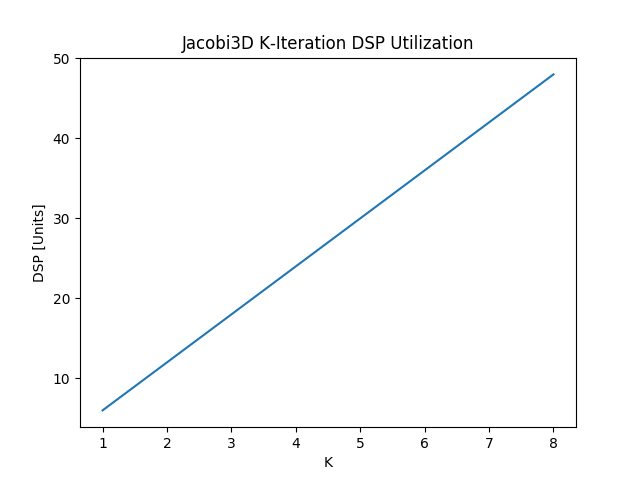
\includegraphics[height=12em]{plots/jacobi3d_k_itr_dsp.png}
	\caption{DSP utilization of k iterations.}
	\label{fig:jacobi3d_k_itr_dsp}
\end{figure}




\paragraph{RAM}

The buffer requirements of Jacobi2D in dimensional form consists of the internal buffer of the kernel only, since a single kernel cannot impose any delay buffers. This is given by $\text{max index} - \text{min index} + 1 = [2, 0, 1]$ which leads to a buffer requirement of
\begin{align}
1 + X*Y*2
\end{align}

\begin{figure}[h]
	\centering
	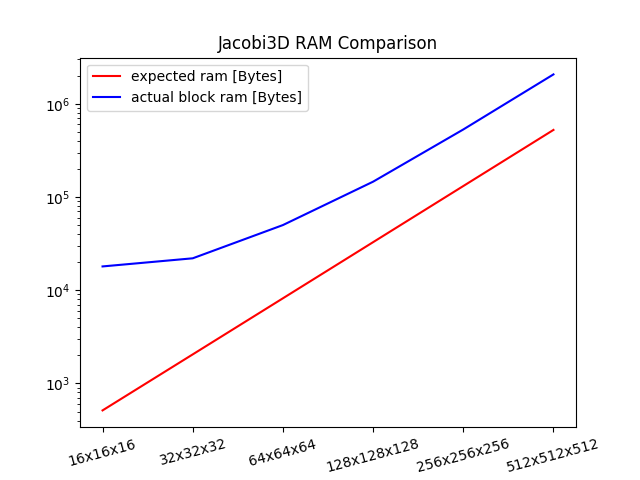
\includegraphics[height=12em]{plots/jacobi3d_ram_comparison.png}
	\caption{Expected buffer size vs block ram usage.}
	\label{fig:jacobi3d_ram_comparison}
\end{figure}

For the K-Iteration case, the RAM amount should grow linear in K by the number of a single Jacobi3D kernel. This is the case as you can see in figure XY.
\begin{figure}[h]
	\centering
	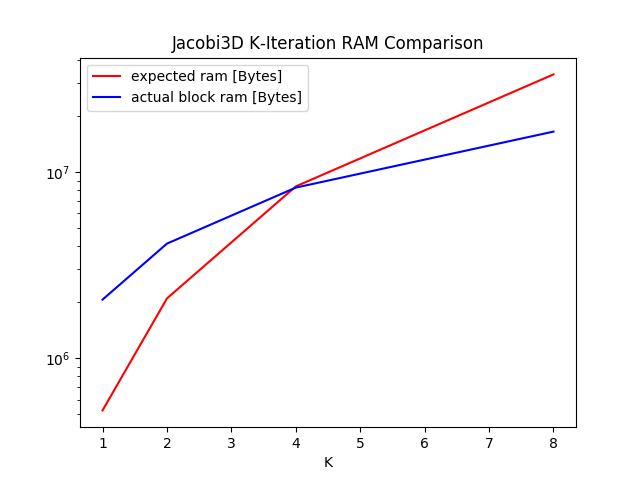
\includegraphics[height=12em]{plots/jacobi3d_ram_comparison_k_iter.png}
	\caption{Expected buffer size vs block ram usage.}
	\label{fig:jacobi3d_ram_comparison_k_iter}
\end{figure}



\paragraph{Execution Time}

In general, the execution time of a pipeline expressed in cycles is given by
\begin{align}
\text{execution time} = D + (N-1)*I
\end{align}
By assuming $I=1$  (producing a result every cycle) and using D as the latency computed by StencilFlow which , our estimate is almost perfectly equal to the measurements, especially for larger problem sizes where we can measure more exact.
\begin{figure}[h]
	\begin{minipage}{.5\columnwidth}
		\centering
		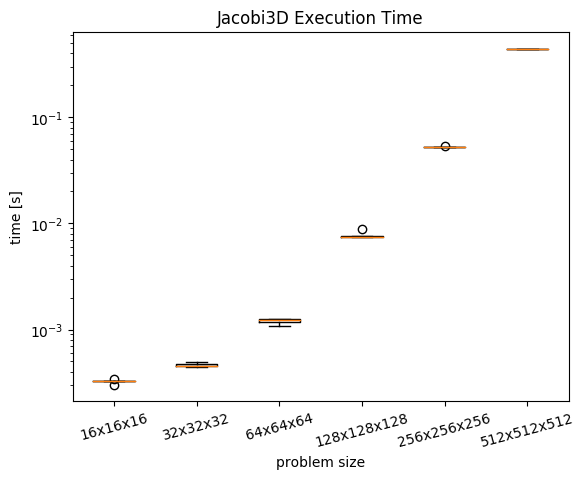
\includegraphics[height=12em]{plots/jacobi3d_execution_time.png}
		\caption{Execution time of Jacobi3D.}
		\label{fig:jacobi3d_execution_time}
	\end{minipage}
	\begin{minipage}{.5\columnwidth}
		\centering
		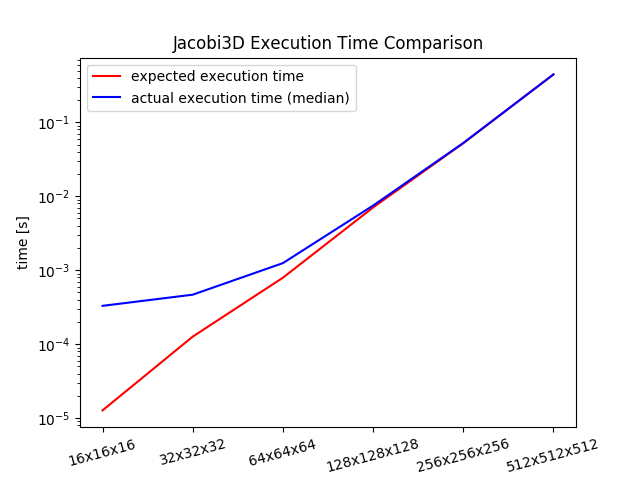
\includegraphics[height=12em]{plots/jacobi3d_execution_time_comparison.png}
		\caption{Expected vs actual execution time.}
		\label{fig:jacobi3d_execution_time}
	\end{minipage}
\end{figure}

The same applies for the K-Iteration case with the modified formula:
\begin{align}
\text{execution time} = K*D + (N-1)*I
\end{align}
\begin{figure}[h]
	\begin{minipage}{.5\columnwidth}
		\centering
		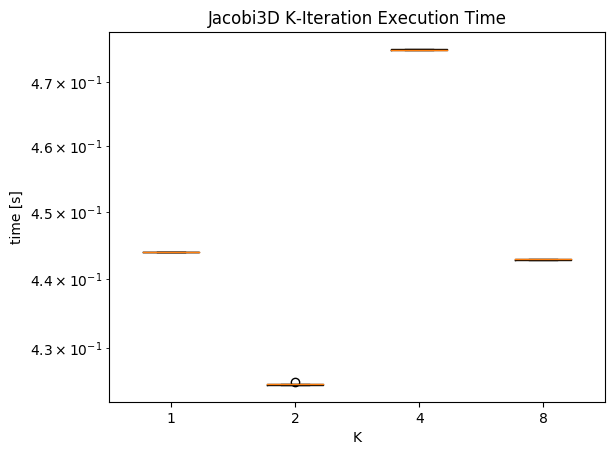
\includegraphics[height=12em]{plots/jacobi3d_execution_time_k_iter.png}
		\caption{Execution time of K-Iteration Jacobi3D.}
		\label{fig:jacobi3d_execution_time_k_iter}
	\end{minipage}
	\begin{minipage}{.5\columnwidth}
		\centering
		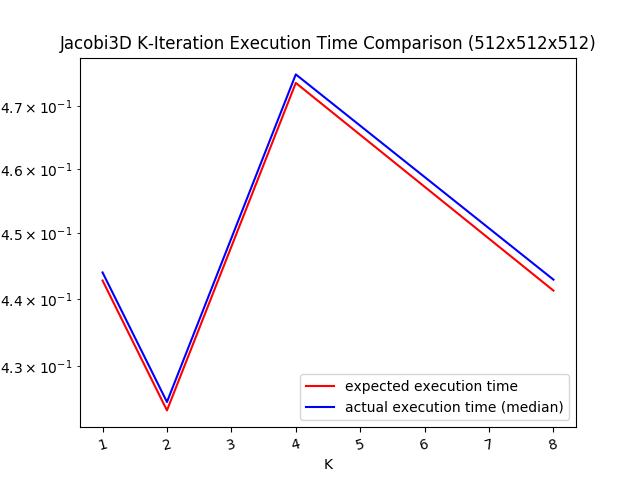
\includegraphics[height=12em]{plots/jacobi3d_execution_time_k_iter_comparison.png}
		\caption{Expected vs actual execution time.}
		\label{fig:jacobi3d_execution_time_k_iter_comparison}
	\end{minipage}
\end{figure}
\\
\textit{Note: The spikes in figure \ref{fig:jacobi3d_execution_time_k_iter} and \ref{fig:jacobi3d_execution_time_k_iter_comparison}  are occurring because of the different HLS design frequencies which accounts much higher compared to the little additional depth the iterations add.}





\section{COSMO Stencil Chains}

\subsection{Fastwaves} 
The fastwaves stencil chain is part of the dynamical core of COSMO. Due to non-disclosure agreement restrictions, we cannot publish the kernel expressions, but we will use the output of StencilFlow for comparison with the measurements from the report and timings from the actual executions.

\begin{figure}[h]
	\centering
	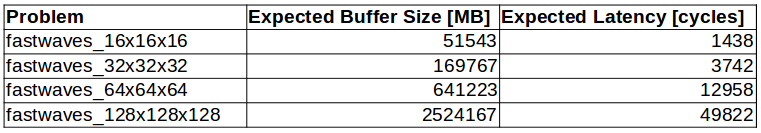
\includegraphics[height=5em]{images/fastwaves-buffer-latency.png}
	\caption{Expected Buffer and Latency from StencilFlow.}
	\label{fig:fastwaves-buffer-latency}
\end{figure}

\paragraph{Frequency}
The design frequency of all problem sizes are between 220Mhz and 260Mhz as we expected. Since these stencil programs have a higher degree of complexity compared to the Jacobi examples, we also expected the frequency to be a bit lower. 


\paragraph{DSP}
The reported number of DSP units is 66 throughout all problem sizes of fast waves, which is what we expected. Since there are 44 additions/subtractions and 28 multiplications/divisions in the kernels of this stencil program, this number is again lower than the sum of 44 and 28. Since the single precision DSP blocks incorporate an add and a multiply unit and shown in figure \ref{fig:stratix10-add-mult}, they might be used concurrently.

\begin{figure}[h]
	\begin{minipage}{.5\columnwidth}
	\centering
	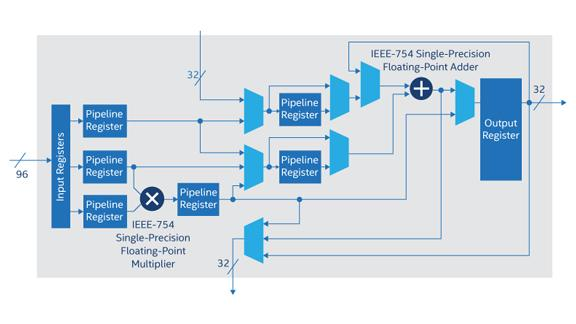
\includegraphics[width=16em]{images/stratix10-add-mult.jpg}
	\caption{Single-Precision Floating Point DSP Block \textit{intel.com}}
	\label{fig:stratix10-add-mult}
	\end{minipage}
	\begin{minipage}{.5\columnwidth}
	\centering
	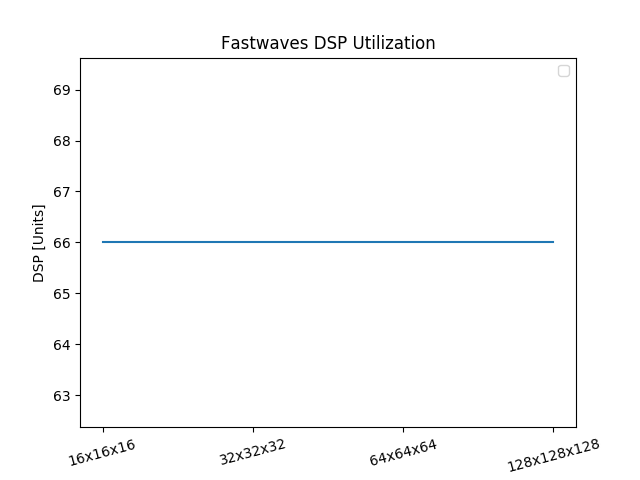
\includegraphics[height=12em]{plots/fastwaves_dsp.png}
	\caption{DSP utilization.}
	\label{fig:fastwaves_dsp}
	\end{minipage}
\end{figure}

\paragraph{RAM}
This design imposes internal and delay buffers of various sizes, which is automatically handled and computed by StencilFlow. We can therefore directly compare the theoretical value to the number we are getting in the report.
\begin{figure}[h]
	\centering
	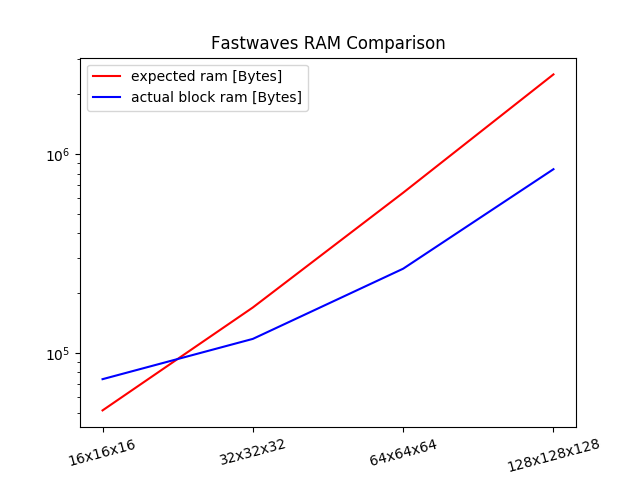
\includegraphics[height=12em]{plots/fastwaves_ram_comparison.png}
	\caption{Expected buffer size vs block ram usage.}
	\label{fig:fastwaves_ram_comparison}
\end{figure}



\paragraph{Execution Time}
In general, the execution time of a pipeline expressed in cycles is given by
\begin{align}
\text{execution time} = D + (N-1)*I
\end{align}
By assuming $I=1$  (producing a result every cycle, shown as approximative value in the report) and using D as the latency computed by StencilFlow, our estimate is about 20-30\% lower.

\begin{figure}[h]
	\begin{minipage}{.5\columnwidth}
		\centering
		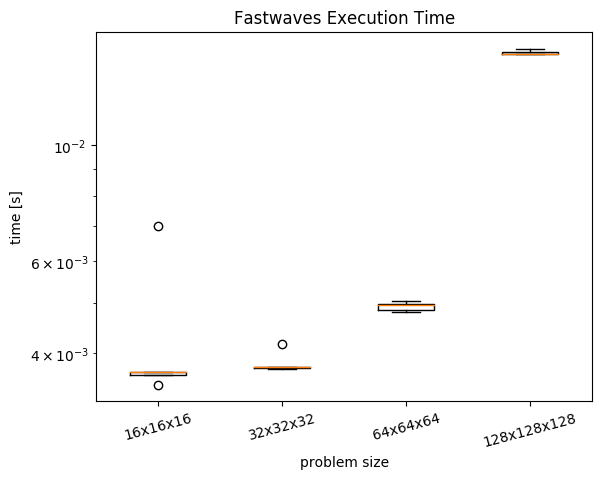
\includegraphics[height=14em]{plots/fastwaves_execution_time.png}
		\caption{Execution time of Fastwaves.}
		\label{fig:fastwaves_execution_time}
	\end{minipage}
	\begin{minipage}{.5\columnwidth}
		\centering
		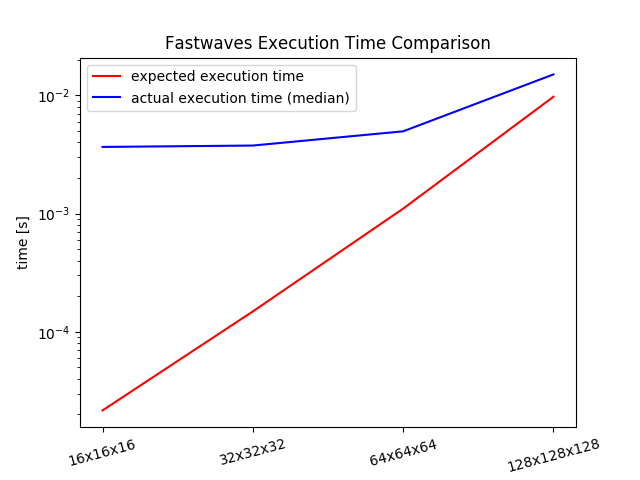
\includegraphics[height=14em]{plots/fastwaves_execution_time_comparison.png}
		\caption{Expected vs actual execution time.}
		\label{fig:fastwaves_execution_time_comparison}
	\end{minipage}
\end{figure}



\subsection{Diffusion} 
The diffusion stencil chain is part of the dynamical core of COSMO. We will use the output of StencilFlow for comparison with the measurements from the report and timings from the actual executions.

\begin{figure}[h]
	\centering
	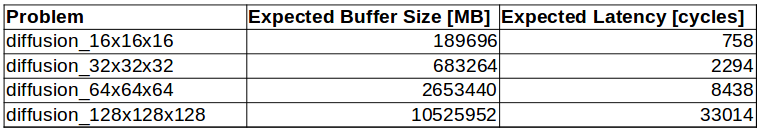
\includegraphics[height=5em]{images/diffusion-buffer-latency.png}
	\caption{Expected Buffer and Latency from StencilFlow.}
	\label{fig:diffusion-buffer-latency}
\end{figure}


\paragraph{Frequency}
The design frequency of all problem sizes are between 260Mhz and 270Mhz as we expected. Since these stencil programs have a higher degree of complexity compared to the Jacobi examples, we also expected the frequency to be a bit lower. 



\paragraph{DSP}
The reported number of DSP units is 56 throughout all problem sizes of diffusion. Since there are 50 additions/subtractions and 17 multiplications/divisions and 9 ternary operator in the kernels of this stencil program, this number is again lower than the sum of 50 and 17. Since the single precision DSP blocks incorporate an add and a multiply unit and shown in figure \ref{fig:stratix10-add-mult}, we conclude that they might be in concurrent use.
%\begin{figure}[h]
%	\centering
%	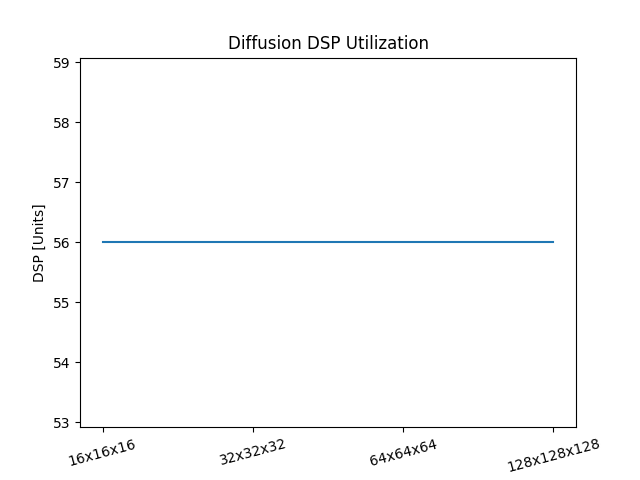
\includegraphics[height=12em]{plots/diffusion_dsp.png}
%	\caption{DSP utilization.}
%	\label{fig:diffusion_dsp}
%\end{figure}

\paragraph{RAM}
This design imposes internal and delay buffers of various sizes, which is automatically handled and computed by StencilFlow. We can therefore directly compare the theoretical value to the number we are getting in the report.\\
\begin{figure}[h]
	\centering
	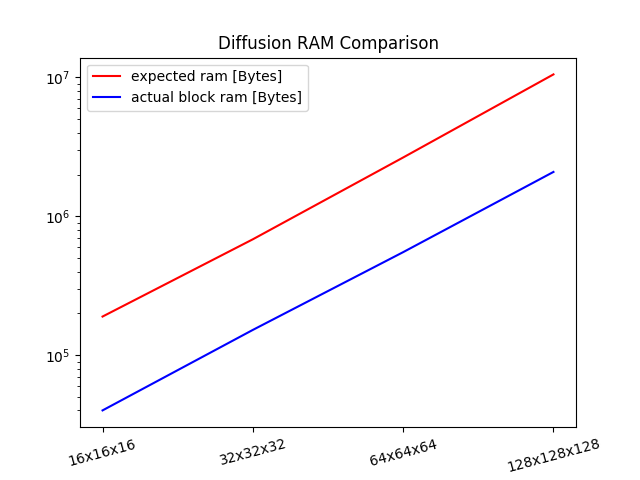
\includegraphics[height=12em]{plots/diffusion_ram_comparison.png}
	\caption{Expected buffer size vs block ram usage.}
	\label{fig:diffusion_ram_comparison}
\end{figure}


\paragraph{Execution Time}
By assuming $I=1$  (producing a result every cycle, shown as approximative value in the report) and using D as the latency computed by StencilFlow, our estimate is about 20-30\% lower.
\begin{figure}[h]
	\begin{minipage}{.5\columnwidth}
		\centering
		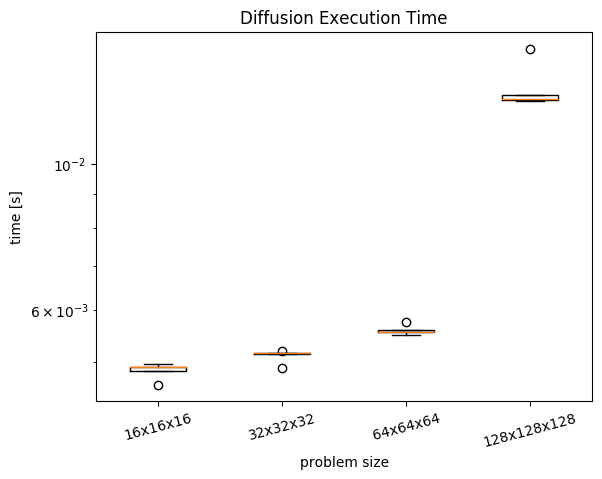
\includegraphics[height=16em]{plots/diffusion_execution_time.png}
		\caption{Execution time of diffusion.}
		\label{fig:diffusion_execution_time}
	\end{minipage}
	\begin{minipage}{.5\columnwidth}
		\centering
		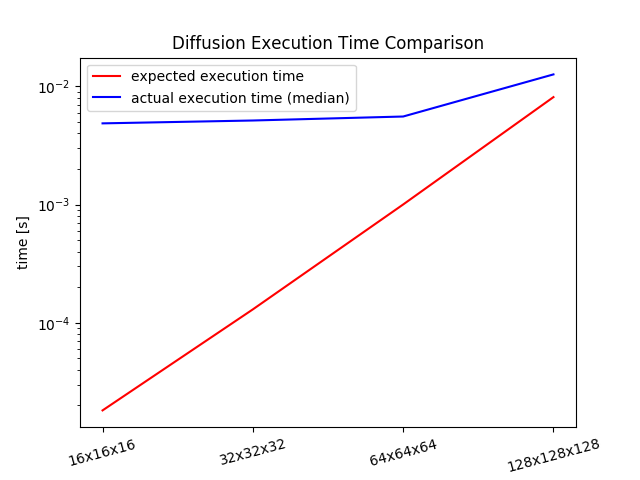
\includegraphics[height=16em]{plots/diffusion_execution_time_comparison.png}
		\caption{Expected vs actual execution time.}
		\label{fig:diffusion_execution_time_comparison}
	\end{minipage}
\end{figure}



\section{Conclusion} 
Most of our theoretical findings correlate very well with the measurements and reports from the real hardware. This builds a good foundation for further investigation into deeper analysis and optimization for the specific platforms. 

